\documentclass[border=10pt]{standalone}
\usepackage[utf8]{inputenc}
\usepackage{tikz}
\usetikzlibrary{shapes.geometric, arrows.meta, positioning, fit, backgrounds, calc}

\definecolor{outerblue}{HTML}{1D0572}
\definecolor{innergreen}{HTML}{1DAB51}
\definecolor{accentgold}{HTML}{CA8919}
\definecolor{lightbg}{HTML}{F1F5F9}
\definecolor{darktext}{HTML}{1E293B}

\begin{document}
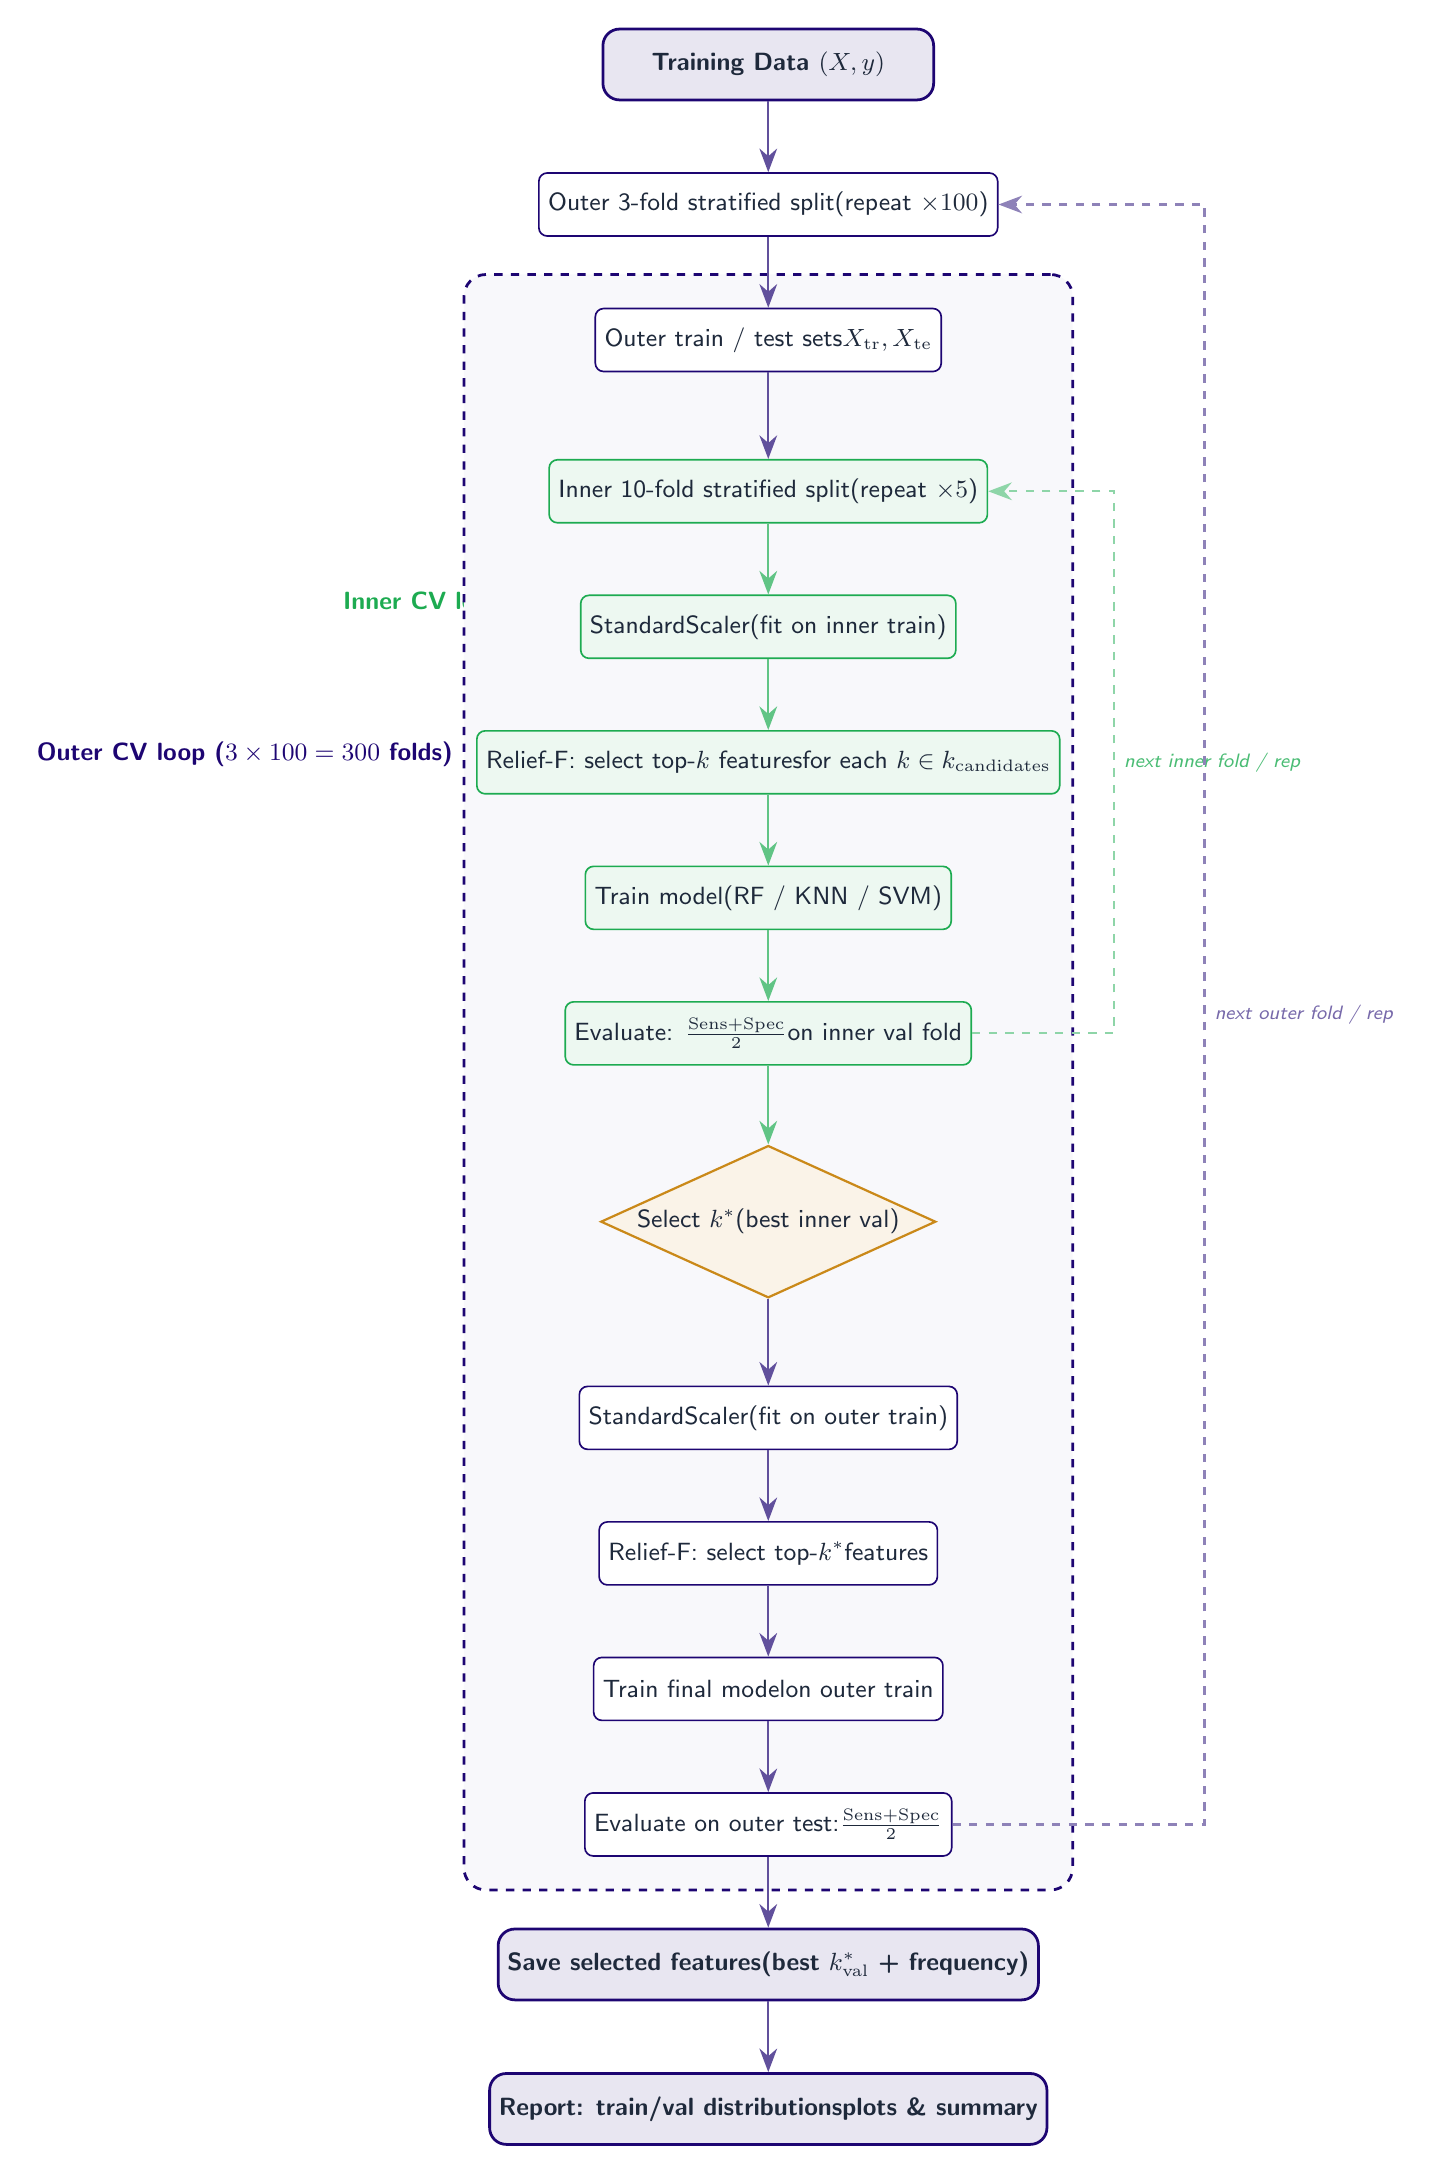
\begin{tikzpicture}[
    node distance=0.9cm and 1.2cm,
    >={Stealth[length=3mm]},
    % --- node styles ---
    startstop/.style={
        rectangle, rounded corners=6pt, minimum width=4.2cm, minimum height=0.9cm,
        text centered, draw=outerblue, line width=1pt,
        fill=outerblue!10, text=darktext, font=\sffamily\bfseries\small
    },
    process/.style={
        rectangle, rounded corners=3pt, minimum width=4.2cm, minimum height=0.8cm,
        text centered, draw=outerblue, line width=0.6pt,
        fill=white, text=darktext, font=\sffamily\small
    },
    innerprocess/.style={
        rectangle, rounded corners=3pt, minimum width=3.6cm, minimum height=0.8cm,
        text centered, draw=innergreen, line width=0.6pt,
        fill=innergreen!8, text=darktext, font=\sffamily\small
    },
    decision/.style={
        diamond, minimum width=3.4cm, minimum height=1.6cm,
        text centered, draw=accentgold, line width=0.8pt,
        fill=accentgold!10, text=darktext, font=\sffamily\small,
        inner sep=1pt, aspect=2.2
    },
    arrow/.style={->, thick, color=outerblue!70},
    innerarrow/.style={->, thick, color=innergreen!70},
    loopback/.style={->, thick, color=outerblue!50, dashed},
    innerloopback/.style={->, thick, color=innergreen!50, dashed},
]

% ===== DATA =====
\node[startstop] (data) {Training Data $(X, y)$};

% ===== OUTER LOOP =====
\node[process, below=of data] (outersplit) {Outer 3-fold stratified split\\(repeat $\times 100$)};
\draw[arrow] (data) -- (outersplit);

\node[process, below=of outersplit] (outertrain) {Outer train / test sets\\$X_{\mathrm{tr}}, X_{\mathrm{te}}$};
\draw[arrow] (outersplit) -- (outertrain);

% ===== INNER LOOP =====
\node[innerprocess, below=1.1cm of outertrain] (innersplit) {Inner 10-fold stratified split\\(repeat $\times 5$)};
\draw[arrow] (outertrain) -- (innersplit);

\node[innerprocess, below=of innersplit] (scale1) {StandardScaler\\(fit on inner train)};
\draw[innerarrow] (innersplit) -- (scale1);

\node[innerprocess, below=of scale1] (relief1)
    {Relief-F: select top-$k$ features\\for each $k \in k_{\mathrm{candidates}}$};
\draw[innerarrow] (scale1) -- (relief1);

\node[innerprocess, below=of relief1] (traininner) {Train model\\(RF / KNN / SVM)};
\draw[innerarrow] (relief1) -- (traininner);

\node[innerprocess, below=of traininner] (evalinner)
    {Evaluate: $\frac{\mathrm{Sens} + \mathrm{Spec}}{2}$\\on inner val fold};
\draw[innerarrow] (traininner) -- (evalinner);

\node[decision, below=1cm of evalinner] (bestk) {Select $k^*$\\(best inner val)};
\draw[innerarrow] (evalinner) -- (bestk);

% inner loop-back arrow
\draw[innerloopback]
    (evalinner.east) -- ++(1.8,0) |- (innersplit.east)
    node[pos=0.25, right, font=\sffamily\scriptsize\itshape, text=innergreen!80] {next inner fold / rep};

% ===== OUTER — FINAL MODEL =====
\node[process, below=1.1cm of bestk] (scale2) {StandardScaler\\(fit on outer train)};
\draw[arrow] (bestk) -- (scale2);

\node[process, below=of scale2] (relief2) {Relief-F: select top-$k^*$\\features};
\draw[arrow] (scale2) -- (relief2);

\node[process, below=of relief2] (trainouter) {Train final model\\on outer train};
\draw[arrow] (relief2) -- (trainouter);

\node[process, below=of trainouter] (evalouter)
    {Evaluate on outer test:\\$\frac{\mathrm{Sens} + \mathrm{Spec}}{2}$};
\draw[arrow] (trainouter) -- (evalouter);

% outer loop-back arrow
\draw[loopback]
    (evalouter.east) -- ++(3.2,0) |- (outersplit.east)
    node[pos=0.25, right, font=\sffamily\scriptsize\itshape, text=outerblue!60] {next outer fold / rep};

% ===== SAVE FEATURES =====
\node[startstop, below=of evalouter] (save)
    {Save selected features\\(best $k^*_{\mathrm{val}}$ + frequency)};
\draw[arrow] (evalouter) -- (save);

% ===== RESULT =====
\node[startstop, below=of save] (result)
    {Report: train/val distributions\\plots \& summary};
\draw[arrow] (save) -- (result);

% ===== BACKGROUND BOXES =====
\begin{scope}[on background layer]
    % Inner loop box
    \node[
        draw=innergreen, dashed, line width=1pt, rounded corners=6pt,
        fill=innergreen!4,
        fit=(innersplit)(evalinner)(bestk),
        inner xsep=12pt, inner ysep=10pt,
        label={[font=\sffamily\bfseries\small, text=innergreen]above left:Inner CV loop}
    ] (innerbox) {};

    % Outer loop box
    \node[
        draw=outerblue, dashed, line width=1pt, rounded corners=8pt,
        fill=outerblue!3,
        fit=(outertrain)(innerbox)(scale2)(relief2)(trainouter)(evalouter),
        inner xsep=18pt, inner ysep=12pt,
        label={[font=\sffamily\bfseries\small, text=outerblue]above left:Outer CV loop ($3 \times 100 = 300$ folds)}
    ] (outerbox) {};
\end{scope}

\end{tikzpicture}
\end{document}
